\chapter{Entwicklung des Konzepts}

In diesem Kapitel wird der Übergang von der Problemanalyse zur kreativen Konzeptentwicklung im Forschungsprozess hervorgehoben. Es markiert die zentrale Phase, in der theoretisches Wissen und praktische Erkenntnisse zusammenfließen, um innovative Lösungsansätze zu formulieren. Wir integrieren theoretische Grundlagen und Modelle aus vorangegangenen Kapiteln und erläutern die angewandten Methoden zur Entwicklung tragfähiger Lösungen. Dieses Kapitel dient als Brücke zwischen Analyse und Umsetzung, betont die kreative Synthese von Ideen und Lösungsansätzen und bietet einen detaillierten Einblick in den Prozess der Konzeptentwicklung.

\section{Verschiedene Herangehensweisen}

Vor der Ausarbeitung des endgültigen Implementierungskonzepts wurden mehrere methodische Ansätze einer eingehenden Untersuchung unterzogen. Das vorrangige Ziel dieser methodischen Herangehensweisen bestand in der Extraktion einer Reihe von Regelwerken, die später in GReQL-Ausdrücke transformiert werden sollten. Diese Regelwerke sollten aus den Kommentaren oder Anmerkungen extrahiert werden, welche von Lehrkräften in Bezug auf eine UML-Übung hinterlassen wurden. Die Wahl des Notenformats ist frei, was viele Möglichkeiten bietet. 

\subsection{YAML-basierten Annotationen}

Der erste untersuchte methodische Ansatz fokussierte auf die Entwicklung eines benutzerfreundlichen Annotationsystems, das eine umfassende Modellierung der Interaktionen innerhalb eines UML-Diagramms ermöglichen sollte. Infolgedessen wurden editierbare Regelobjekte abgeleitet, welche aus diesem Annotationsystem generiert wurden. Sobald der Nutzer sämtliche Regeln, die aus dem Annotationsystem resultierten, verifizierte, konnte er GReQL-Code generieren, welcher anschließend in das JACK-System eingefügt wurde. Die Konzeption dieses schlichten Notationssystems diente dem Zweck der Abbildung von Beziehungen innerhalb eines UML Klassendiagramms. Zu diesem Zweck wurde das YAML-Format aus mehreren Gründen präferiert:

\begin{enumerate}
    \item Erstens, das Schreiben im YAML-Format erweist sich als unkompliziert.
    \item Zweitens, es liefert Daten in einem strukturierten Format, welches leicht manipuliert werden kann.
\end{enumerate}


\begin{figure}
	\centering
	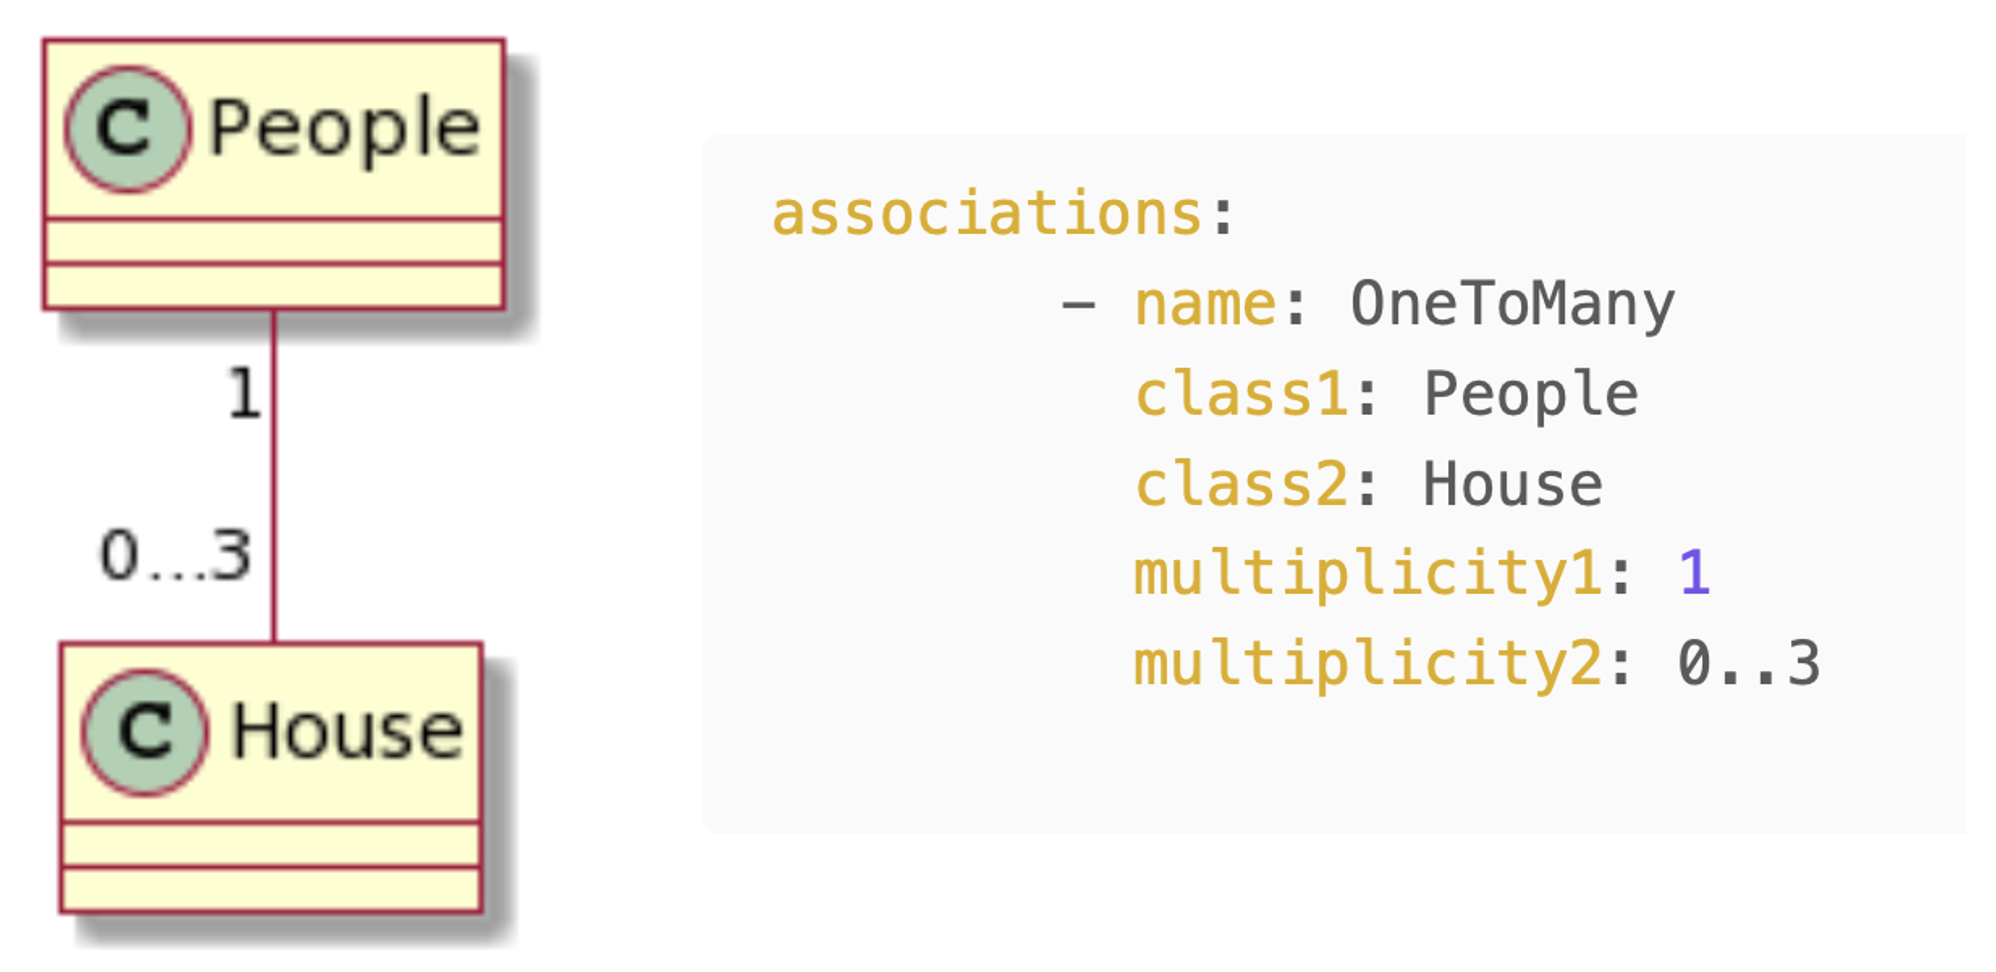
\includegraphics[width=15cm]{images/yaml-uml.png}
	\caption{Beispiel einer Annotation von UML mit YAML}
	\label{fig:yaml-uml}
\end{figure}


Die Notation in YAML mag den Eindruck vermitteln, bereits eine Form der Regeldefinition darzustellen, weil der Lehrende bereits alle Interaktionen zwischen den verschiedenen Objekten im Diagramm definiert. Um jedoch die Klarheit bezüglich dieser Frage zu gewährleisten, könnte es sinnvoll sein, ein weniger formelles Notationssystem zu etablieren. Beispielweise:

\begin{itemize}
    \item Die Klasse A erbt von der Klasse B.
    \item Die Klasse A besitzt drei Attribute:
    \begin{itemize}
        \item Attribut a vom Typ x mit öffentlicher Sichtbarkeit.
        \item Attribut b vom Typ y mit öffentlicher Sichtbarkeit.
        \item Attribut c vom Typ z mit privater Sichtbarkeit.
    \end{itemize}
\end{itemize}

oder ein noch weniger wortreiches System: 

\begin{itemize}
    \item A $\Rightarrow$ B 
    \item A:
    \begin{itemize}
        \item +a:x (+ für öffentlich)
        \item +b:y
        \item -c:z (- für privat)
    \end{itemize}
\end{itemize}


Dieses System ähnelt eher herkömmlichen Kommentaren, jedoch könnte es herausfordernder sein, den darin enthaltenen Text zu analysieren und daraus anwendbare Regelvorschläge zu extrahieren. Trotzdem birgt dieser methodische Ansatz mehrere Limitationen:

\begin{enumerate}
    \item Es existieren bereits seit geraumer Zeit vielfältige Notationssysteme und Datenformate für UML, wie beispielsweise XMI \cite{skogan1999uml}, \ac{UXF} \cite{suzuki1998making}, Textbasierte \cite{washizaki2010tcd} oder JSON-basierte Datenformate \cite{benson2021uml}, um nur einige zu nennen.

    \item Die Entwicklung eines vollständig neuen und umfassenden Notationssystems innerhalb eines begrenzten Zeitraums kann äußerst zeitintensiv sein, insbesondere wenn es die umfassende Darstellung sämtlicher Varianten eines UML-Klassendiagramms anstrebt.

    \item Dieses System verlagert die Aufgabe der Ableitung von Beziehungen zwischen den verschiedenen Objekten lediglich in ein anderes Format, ohne dabei die Arbeitsbelastung für die Lehrkraft zu mindern.
\end{enumerate}


In Anbetracht dieser diversen Überlegungen wurde von der Verfolgung dieses methodischen Ansatzes Abstand genommen, und es erfolgte die Exploration alternativer Vorgehensweisen.


\subsection{Verwendung von Natural Language Processing  Tools}

Die zweite konzeptionelle Idee besteht darin, ein \ac{NLP}-Tool zu verwenden, um die Kommentare oder Notizen des Lehrers zu analysieren. Anschließend kann das NLP-Tool verwendet werden, um Empfehlungen auf der Grundlage einer vorher festgelegten Reihe von Parametern für den Lehrer abzugeben. Diese Parameter könnten eine Reihe von UML-Regeln in einem spezifischen Format sein, so dass die KI in der Lage ist, die richtige Lösung auf der Grundlage des Kommentars zu finden. Der Vorschlag könnte dann in GReQL-Code übersetzt werden. Diese Herangehensweise hat jedoch auch einige Herausforderungen:

\begin{enumerate}
    \item Die von dieser Methode generierten Lösungen neigen dazu, ungenau zu sein, und es sind möglicherweise zahlreiche Anpassungen erforderlich, um das gewünschte Ergebnis zu erzielen \cite{chowdhary2020natural}. Dies könnte möglicherweise die Arbeitsbelastung der Lernenden erhöhen, anstatt sie zu erleichtern.
    \item Es wäre notwendig, die KI darauf zu trainieren, bestimmte Muster zu erkennen und sie mit vordefinierten Regeln in Verbindung zu bringen, um die Zuverlässigkeit zu erhöhen.

\end{enumerate}

In ihrem aktuellen Stand erfordert diese Herangehensweise erhebliche Anstrengungen, um diese Herausforderungen zu bewältigen und eine effektive Implementierung zu erreichen. Aufgrund der potenziellen Schwierigkeiten bei der Implementierung und der möglicherweise nicht zufriedenstellenden Ergebnisse wurde dieser Ansatz auch aufgegeben.

\section{Konzept}\label{sec:konzept}

Bei der Entwicklung des Konzepts wurde ein radikal andersartiger Ansatz als der in dem vorherigen Abschnitt dargelegte verfolgt. Die Herangehensweise, Regeln aus Kommentaren abzuleiten, erweist sich als ein komplexer Prozess und potenziell schwierig umzusetzen. Die Gewährleistung der Zuverlässigkeit der erzielten Ergebnisse stellt ebenfalls eine bedeutende Herausforderung dar. In diesem Zusammenhang wurde eine intuitivere Herangehensweise in Betracht gezogen, nämlich die direkte Ableitung von Regeln aus der Mustervorlage.

Bevor dieses Konzept im Detail beschrieben wird, ist es unerlässlich, das Endziel in Erinnerung zu rufen, nämlich die Unterstützung von Lehrenden bei der Bewertung von UML-Übungsaufgaben (insbesondere Klassendiagrammen). Dies soll durch erhebliche Vereinfachung des Schreibens von GReQL-Code auf der JACK-Plattform erreicht werden, indem Lehrern mit Hilfe eines im Rahmen dieser Masterarbeit zu entwickelnden Tools (halb-)automatische Unterstützung geboten wird. Das Konzept zur Erfüllung dieser Aufgabe kann in drei Wichtige Schritte unterteilt werden:

\subsubsection{Schritt 1: Erstellung einer Musterlösung mit Hilfe eines Modellierungstools}

Wie im \autoref{sec:bewertungsprozess} erwähnt wurde, umfasst Phase 2 die optionalen Schritte zur Erstellung einer Musterlösung. In diesem Konzept ist diese Phase unerlässlich und gewinnt ihre volle Bedeutung. Nachdem ein UML-Klassendiagrammübungsaufgabe entwickelt wurde, erstellen die meisten Lehrer eine Musterlösung, oft in Form eines Klassendiagramms. Diese Lösung wird dann mit den verschiedenen Einreichungen der Studenten verglichen, und Punkte werden gemäß den vom Lehrer festgelegten Kriterien an die einzelnen Studenten vergeben. Da in den meisten Fällen eine Musterlösung in Form eines Klassendiagramms für die Aufgabe vorhanden ist, wäre es sinnvoll, diese zur Ableitung relevanter Regeln zu verwenden. Dies stellt die erste Phase des Ansatzes dar, bei der eine Musterlösung mithilfe einer Modellierungsanwendung erstellt wird, die anschließend die Möglichkeit bietet, das Diagramm in einem leicht programmierbaren Format zu exportieren.

\subsubsection{Schritt 2: Verarbeitung der exportierten Datei}

Nachdem der Lehrer die Musterlösung erfolgreich modelliert hat, ergibt sich die Notwendigkeit, diese Vorlage in ein geeignetes Format zu exportieren, welches eine programmgesteuerte Bearbeitung ermöglicht. Dieser Transformationsprozess kann mittels diverser Datenformate wie JSON, XML oder sogar YAML realisiert werden. Sobald das exportierte Dokument verfügbar ist, eröffnet sich im Kontext eines Klassendiagramms die Möglichkeit, zunächst sämtliche in der Musterlösung enthaltenen Klassen sowie sämtliche Interdependenzen zwischen den verschiedenen Elementen zu extrahieren. Infolge dieses Phasenschritts besteht die Option zur Ableitung von ``Regel''-Objekten, welche auf der Frontend-Oberfläche sichtbar sind und vom Lehrer interaktiv bearbeitet werden können. Die Bereitstellung dieser Funktionalität befähigt den Lehrer dazu, wertvolles Feedback hinzuzufügen, die zugehörigen Punktzahlen zu definieren und sämtliche erforderlichen Informationen für den nächsten Schritt und die anschließende Evaluierung umfassend zu vervollkommnen.

\subsubsection{Schritt 3: Generierung des GReQL-Codes}

Der abschließende Schritt dieses Vorgehens umfasst die Generierung von GReQL-Code aus den Regeln, die in der vorherigen Phase extrahiert und/oder hinzugefügt wurden. Nachdem die Konfiguration abgeschlossen ist, muss der GReQL-Code unter Verwendung verschiedener XMI-Vorlagen generiert werden. Der resultierende Code kann vom Lehrer auf der JACK-Plattform verwendet werden.

\begin{figure}
	\centering
	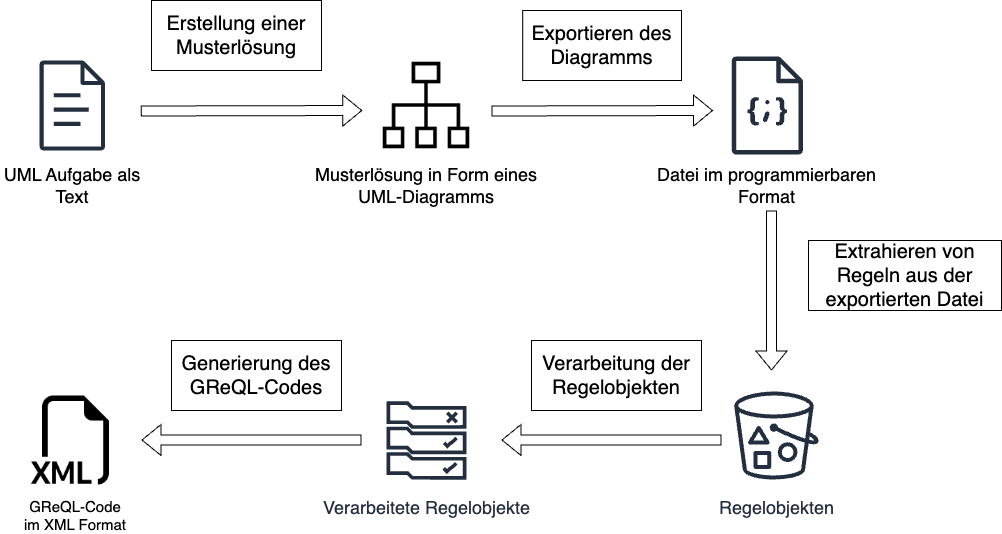
\includegraphics[width=15cm]{images/concept.png}
	\caption{Repräsentatives schema des konzepts.}
	\label{fig:concept}
\end{figure}

Durch dieses Konzept (siehe Abbildung~\ref{fig:concept}) und seine verschiedenen Schritte ist es möglich, von einer Musterlösung zur Generierung des erforderlichen GReQL-Codes für die Bewertung von Diagrammen durch JACK zu gelangen. Dieser Ansatz hat das Potenzial, den Bewertungsprozess von Diagrammen über die JACK-Plattform erheblich zu vereinfachen, was das zentrale Ziel dieser Masterarbeit ist. Die tatsächliche Umsetzung dieses Konzepts hängt jedoch eng vom gewählten Workflow und der Art und Weise ab, wie das Konzept umgesetzt wird. Dieser Ausblick leitet zum nächsten Kapitel über, das die Implementierung behandelt.